\documentclass[11pt]{article}
\usepackage[utf8]{inputenc}

% add LaTeX packages to use here
\usepackage{amsmath}
\usepackage{amssymb}
\usepackage{amsfonts}
\usepackage{amsthm}
\usepackage{fancyhdr}
\usepackage{lastpage}
\usepackage{enumitem}
\usepackage{framed}
\usepackage[most]{tcolorbox}
\usepackage{geometry}
\usepackage{graphicx}

 % set dimensions for page layout
\geometry
{
 left=5em,
 right=5em,
 bottom=5em,
 top=6em,
 headheight=110pt,
 showframe=false
}

\setlist[itemize]{leftmargin=*} % prevents indenting of itemize

% abbreviations for some common math symbols
\newcommand{\Rset}{\hbox{$\mathbb R$}}
\newcommand{\Nset}{\hbox{$\mathbb N$}}
\newcommand{\Pset}{\hbox{$\mathbb{N}^{+}$}}
\newcommand{\Zset}{\hbox{$\mathbb N$}}
\newcommand{\Qset}{\hbox{$\mathbb Q$}}

% theorem style
\newtheoremstyle{thmstyle}% name of the style to be used
  {0pt}% measure of space to leave above the theorem. E.g.: 3pt
  {0pt}% measure of space to leave below the theorem. E.g.: 3pt
  {}% name of font to use in the body of the theorem
  {}% measure of space to indent
  {\bfseries}% name of head font
  {.}% punctuation between head and body
  { }% space after theorem head; " " = normal inter-word space
  {}% Manually specify head

% theorem environment instance
\theoremstyle{thmstyle}
\newtheorem{theorem}{Theorem}

% shaded and framed solution environment 
\makeatletter
\newenvironment{shadedSolutionBox}
  {\setlength{\OuterFrameSep}{0in}%
  \definecolor{shadecolor}{gray}{.8}% shading of shaded solution box
  \bigskip%
  \@nameuse{shaded*}\par\noindent\ignorespaces \textit{Solution}.}
  {\hspace{\stretch{1}}\rule{1.5ex}{1.5ex}% adds filled box 
  \@nameuse{endshaded*}%
  \bigskip}
\makeatother

% shaded and framed theorem environment 
\makeatletter
\newenvironment{thm}
  {\setlength{\OuterFrameSep}{0in}%
  \definecolor{shadecolor}{gray}{1}% shading of shaded Theorem box
  \@nameuse{snugshade*}\par\noindent\ignorespaces%
   \@nameuse{theorem}}
  {\hspace{\stretch{1}}\scalebox{1.5}{\hbox{$\triangleleft$}}% adds triangle shape
  \@nameuse{endtheorem}%
  \@nameuse{endsnugshade*}%
  }
\makeatother

% header and footer elements of every page except the first.
\pagestyle{fancy}
\fancyfoot[L]{\textsc{CISC {\small\selectfont 3230}} }
\fancyhead[R]{{\small\selectfont\textsc{\studentLastName}}}
\fancyfoot[C]{{\small\selectfont\assignmentName}}
\fancyfoot[R]{{\small\selectfont\thepage\ of \pageref{LastPage}}}
\renewcommand{\headrulewidth}{0.8pt}
\renewcommand{\footrulewidth}{0.4pt}

% hline with variable thickness
\makeatletter
\def\thickhline{%
  \noalign{\ifnum0=`}\fi\hrule \@height \thickarrayrulewidth \futurelet
   \reserved@a\@xthickhline}
\def\@xthickhline{\ifx\reserved@a\thickhline
               \vskip\doublerulesep
               \vskip-\thickarrayrulewidth
             \fi
      \ifnum0=`{\fi}}
\makeatother

% length instance for \thickhline
\newlength{\thickarrayrulewidth} 
\setlength{\thickarrayrulewidth}{.8pt}

% header and footer for first page
\fancypagestyle{firstpage}
{
\fancyhf{}
\renewcommand{\footrulewidth}{0.4pt}
\renewcommand{\headrulewidth}{0pt}
\fancyhead[C]{%
\begin{tabular*}{\textwidth}{@{\extracolsep{\fill}}@{}l @{} c @{} r @{} }
{\small\selectfont\courseName}&{\normalsize\selectfont\assignmentName}&{\small\selectfont\studentFirstName\ \studentLastName}\\
\thickhline
&&{\scriptsize\selectfont\collaboratorNames}
\end{tabular*}%
}
\fancyfoot[R]{{\small\selectfont\thepage\ of \pageref{LastPage}}}
\fancyfoot[L]{{\footnotesize\selectfont\pdfcreationdate}}
}

\newcommand{\courseName}{Theoretical Computer Science} % course name

% your first name, your last name, and the assignment name
\newcommand{\studentLastName}{Nikabadze} % your last name
\newcommand{\studentFirstName}{Luka} % your first name (and middle name, if applicable)
\newcommand{\assignmentName}{Homework 1 part 1} % the assignment name
\newcommand{\collaboratorNames}{[First Name Initial]. Last Name} % if you worked with anyone to complete any part of the assignment, include the initial of the first name (and middle name, if applicable) and full last name of each of your collaborators, separated by commas (e.g., if you worked with Arthur Paul Pedersen and Sandra Lee, include "A.P. Pedersen, S. Lee")




\begin{document} % marks the beginning of the document

\thispagestyle{firstpage} % institutes page style for first page

\setlength{\abovedisplayskip}{20pt} % space above math in align* environment
\setlength{\belowdisplayskip}{20pt} % space below math in align* environment



% marks the beginning of the document body


\begin{itemize}\setlength{\itemsep}{1em} % \itemsep is the spacing between items in environment
\item[1.]  First let define M $(Q, \sum, \delta, q_0, F)$ is a DFA of A. Lets build NFA M' for $A^R$ with the following steps: 

{\text{Reverse all arrows }}

{\text{Convert start state for M as the only accept state for M' }}

{\text{Add new start state for M' and for $ q_0'$ }}

{\text{Graph M }}



\begin{document}

\begin{center}
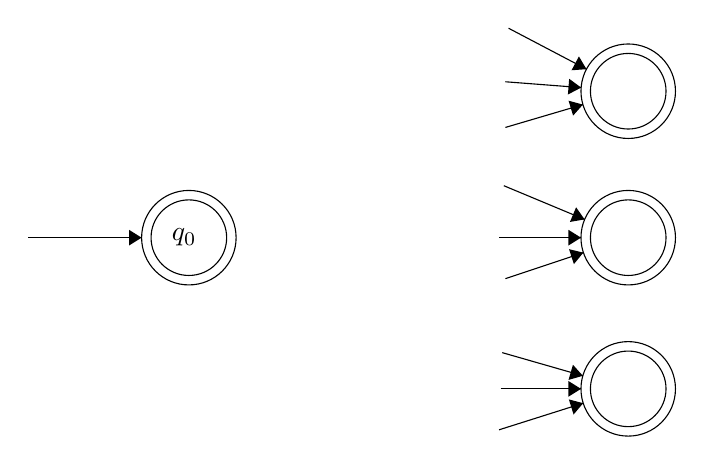
\begin{tikzpicture}[scale=0.2]
\tikzstyle{every node}+=[inner sep=0pt]
\draw [black] (23.1,-25.3) circle (3);
\draw (23.1,-25.3) node {$q_0\mbox{ }$};
\draw [black] (23.1,-25.3) circle (2.4);
\draw [black] (51,-16) circle (3);
\draw [black] (51,-16) circle (2.4);
\draw [black] (51,-25.3) circle (3);
\draw [black] (51,-25.3) circle (2.4);
\draw [black] (51,-34.9) circle (3);
\draw [black] (51,-34.9) circle (2.4);
\draw [black] (12.9,-25.3) -- (20.1,-25.3);
\fill [black] (20.1,-25.3) -- (19.3,-24.8) -- (19.3,-25.8);
\draw [black] (42.9,-34.9) -- (48,-34.9);
\fill [black] (48,-34.9) -- (47.2,-34.4) -- (47.2,-35.4);
\draw [black] (42.8,-37.5) -- (48.14,-35.81);
\fill [black] (48.14,-35.81) -- (47.23,-35.57) -- (47.53,-36.53);
\draw [black] (43,-32.6) -- (48.12,-34.07);
\fill [black] (48.12,-34.07) -- (47.49,-33.37) -- (47.21,-34.33);
\draw [black] (43.2,-27.9) -- (48.15,-26.25);
\fill [black] (48.15,-26.25) -- (47.24,-26.03) -- (47.55,-26.98);
\draw [black] (42.8,-25.3) -- (48,-25.3);
\fill [black] (48,-25.3) -- (47.2,-24.8) -- (47.2,-25.8);
\draw [black] (43.1,-22) -- (48.23,-24.14);
\fill [black] (48.23,-24.14) -- (47.69,-23.37) -- (47.3,-24.3);
\draw [black] (43.2,-18.3) -- (48.12,-16.85);
\fill [black] (48.12,-16.85) -- (47.21,-16.6) -- (47.5,-17.55);
\draw [black] (43.2,-15.4) -- (48.01,-15.77);
\fill [black] (48.01,-15.77) -- (47.25,-15.21) -- (47.17,-16.21);
\draw [black] (43.4,-12) -- (48.35,-14.6);
\fill [black] (48.35,-14.6) -- (47.87,-13.79) -- (47.4,-14.67);
\end{tikzpicture}
\end{center}



{\text{Graph M' }}

\begin{document}

\begin{center}
\begin{tikzpicture}[scale=0.2]
\tikzstyle{every node}+=[inner sep=0pt]
\draw [black] (24.7,-26.6) circle (3);
\draw (24.7,-26.6) node {$q_0$};
\draw [black] (24.7,-26.6) circle (2.4);
\draw [black] (46.7,-25.7) circle (3);
\draw [black] (63.6,-25.7) circle (3);
\draw (63.6,-25.7) node {$q'_0$};
\draw [black] (46.7,-14.4) circle (3);
\draw [black] (47.4,-38.6) circle (3);
\draw [black] (76.2,-25.7) -- (66.6,-25.7);
\fill [black] (66.6,-25.7) -- (67.4,-26.2) -- (67.4,-25.2);
\draw [black] (60.6,-25.7) -- (49.7,-25.7);
\fill [black] (49.7,-25.7) -- (50.5,-26.2) -- (50.5,-25.2);
\draw (55.15,-25.2) node [above] {$\epsilon$};
\draw [black] (61.11,-24.03) -- (49.19,-16.07);
\fill [black] (49.19,-16.07) -- (49.58,-16.93) -- (50.14,-16.1);
\draw (56.07,-19.55) node [above] {$\epsilon$};
\draw [black] (61.25,-27.57) -- (49.75,-36.73);
\fill [black] (49.75,-36.73) -- (50.68,-36.62) -- (50.06,-35.84);
\draw (54.57,-31.66) node [above] {$\epsilon$};
\draw [black] (44.08,-15.85) -- (27.32,-25.15);
\fill [black] (27.32,-25.15) -- (28.27,-25.19) -- (27.78,-24.32);
\draw [black] (43.7,-25.82) -- (27.7,-26.48);
\fill [black] (27.7,-26.48) -- (28.52,-26.94) -- (28.48,-25.95);
\draw [black] (44.75,-37.2) -- (27.35,-28);
\fill [black] (27.35,-28) -- (27.83,-28.82) -- (28.29,-27.93);
\end{tikzpicture}
\end{center}
{\textbf{here $q'_0 = q'_{accept}$.  for any w$\epsilon$ $\sum *$. there is a path following w from the start state to an accept state in M if there is a path following w^R from $q_0'$ to $q'_{accept}$ in M'}}

\item[2.] 
{\textbf{Consider  that $B_n$ is {$a^k$ | k is a multiple of n}
in order to prove that give expression is regular, the value of n is chosen as greater than or equal to 1}}

{\textbf{lets say that $k = ni$, where i is positive integer. lets say that when $i = 1 $ and $n=1$ }}

$B_1 = {a^k}$   \hspace{30}   $B_2 = {a^k}$     \hspace{30}  $B_3 = {a^k}$

$B_1 = {a^{ni}}$ \hspace{27}  $B_2 = {a^{n1}}$    \hspace{25} $B_3 = {a^{n1}}$

$B_1 = {a^{1*1}}$  \hspace{22} $B_2 = {a^{2*1}}$    \hspace{22}  $B_3 = {a^{3*1}}$

$B_1 = {a}$      \hspace{34}  $B_2 = {aa}$   \hspace{32} $B_2 = {aaa}$


{\textbf{now lets build finite automation for the expression }}


\begin{document}

\begin{center}
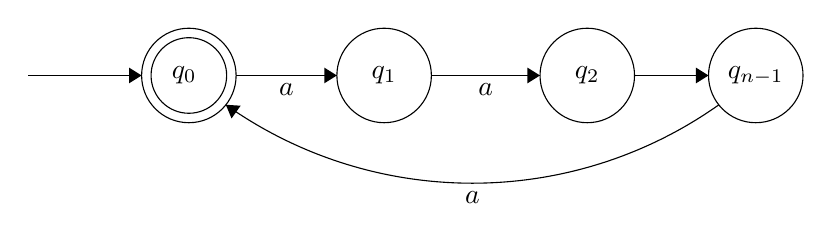
\begin{tikzpicture}[scale=0.2]
\tikzstyle{every node}+=[inner sep=0pt]
\draw [black] (20.5,-25.3) circle (3);
\draw (20.5,-25.3) node {$q_0\mbox{ }$};
\draw [black] (20.5,-25.3) circle (2.4);
\draw [black] (32.9,-25.3) circle (3);
\draw (32.9,-25.3) node {$q_1$};
\draw [black] (45.8,-25.3) circle (3);
\draw (45.8,-25.3) node {$q_2$};
\draw [black] (56.5,-25.3) circle (3);
\draw (56.5,-25.3) node {$q_{n-1}$};
\draw [black] (10.3,-25.3) -- (17.5,-25.3);
\fill [black] (17.5,-25.3) -- (16.7,-24.8) -- (16.7,-25.8);
\draw [black] (23.5,-25.3) -- (29.9,-25.3);
\fill [black] (29.9,-25.3) -- (29.1,-24.8) -- (29.1,-25.8);
\draw (26.7,-25.8) node [below] {$a$};
\draw [black] (48.8,-25.3) -- (53.5,-25.3);
\fill [black] (53.5,-25.3) -- (52.7,-24.8) -- (52.7,-25.8);
\draw [black] (54.152,-27.165) arc (-54.72061:-125.27939:27.1);
\fill [black] (22.85,-27.16) -- (23.21,-28.03) -- (23.79,-27.22);
\draw (38.5,-32.64) node [below] {$a$};
\draw [black] (35.9,-25.3) -- (42.8,-25.3);
\fill [black] (42.8,-25.3) -- (42,-24.8) -- (42,-25.8);
\draw (39.35,-25.8) node [below] {$a$};
\end{tikzpicture}
\end{center}


{\textbf{Union of $B_1$ and ${B_2}$ results in the third string and it is also a regular expression
similarly, if we apply any property of close then the result is regular expression. 
Hence we proved that the above expression is a regular expression}}



\item[3.A] 
 Let say that N= $(Q, \sum, \delta, q_0, F)$ be an NFA with k states that recognizes some language A and lets suppose A is non empty.

Then there must be an accept state that cab be reached from the start state $q_o$ 

Then let w be the string that can be accepted by N when traveling along the shortest path $q_0$ to $q$

Then let n be the length of 2

the sequence of state in the shortest path from $q_0$ to q has length $n+1$

since there are only J states in N that are n distinct states in the shortest path from $q_0$ to q we have $n<k$

so W is accepted by N because q is an accept state

so a contains a string of length at most K


\end{document}
\end{document}
\end{document}
\end{itemize}
\end{document}